%% ****** Start of file apstemplate.tex ****** %
%%
%%
%%   This file is part of the APS files in the REVTeX 4 distribution.
%%   Version 4.1r of REVTeX, August 2010
%%
%%
%%   Copyright (c) 2001, 2009, 2010 The American Physical Society.
%%
%%   See the REVTeX 4 README file for restrictions and more information.
%%
%
% This is a template for producing manuscripts for use with REVTEX 4.0
% Copy this file to another name and then work on that file.
% That way, you always have this original template file to use.
%
% Group addresses by affiliation; use superscriptaddress for long
% author lists, or if there are many overlapping affiliations.
% For Phys. Rev. appearance, change preprint to twocolumn.
% Choose pra, prb, prc, prd, pre, prl, prstab, prstper, or rmp for journal
%  Add 'draft' option to mark overfull boxes with black boxes
%  Add 'showpacs' option to make PACS codes appear
%  Add 'showkeys' option to make keywords appear
\documentclass[aps,prl,twocolumn,superscriptaddress]{revtex4-1}
%\documentclass[aps,prl,preprint,superscriptaddress]{revtex4-1}
%\documentclass[aps,prl,reprint,groupedaddress]{revtex4-1}

% You should use BibTeX and apsrev.bst for references
% Choosing a journal automatically selects the correct APS
% BibTeX style file (bst file), so only uncomment the line
% below if necessary.
\bibliographystyle{apsrev4-1}
%\usepackage{cite}

%\usepackage[english]{babel}
%\usepackage[utf8]{inputenc}
\usepackage{amsmath}
\usepackage{graphicx}
\usepackage{amsfonts}
%\usepackage[colorinlistoftodos]{todonotes}

\usepackage[caption=false]{subfig}
%\usepackage{graphicx}
%\usepackage{caption}
%\usepackage{subcaption}


\newcommand{\vcrm}[1]{\mathbf{#1}}
\newcommand{\hvcrm}[1]{\mathbf{\hat{#1}}}
\newcommand{\vc}[1]{\boldsymbol{#1}}
\newcommand{\hvc}[1]{\boldsymbol{\hat{#1}}}

\newcommand{\ssa}[0]{\sin{\alpha}}
\newcommand{\cca}[0]{\cos{\alpha}}
\newcommand{\ssb}[0]{\sin{\beta}}
\newcommand{\ccb}[0]{\cos{\beta}}
\newcommand{\ssc}[0]{\sin{\gamma}}
\newcommand{\ccc}[0]{\cos{\gamma}}
\newcommand{\sst}[0]{\sin{\theta}}
\newcommand{\cct}[0]{\cos{\theta}}
\newcommand{\ssp}[0]{\sin{\phi}}
\newcommand{\ccp}[0]{\cos{\phi}}

\newcommand{\xsa}[0]{\sin{\alpha}}
\newcommand{\xca}[0]{\cos{\alpha}}
\newcommand{\xsb}[0]{\sin{\beta}}
\newcommand{\xcb}[0]{\cos{\beta}}
\newcommand{\xsc}[0]{\sin{\gamma}}
\newcommand{\xcc}[0]{\cos{\gamma}}
\newcommand{\xst}[0]{\sin{\theta}}
\newcommand{\xct}[0]{\cos{\theta}}
\newcommand{\xsp}[0]{\sin{\phi}}
\newcommand{\xcp}[0]{\cos{\phi}}

\newcommand{\dd}{\mathrm{d}}
\newcommand{\ee}{\mathrm{e}}
\newcommand{\ii}{\mathrm{i}}
\newcommand{\kk}{\mathrm{k}_B}

\newcommand{\vm}{\vc{\mu}}
\newcommand{\vn}{\hvcrm{n}}
\newcommand{\vB}{\vcrm{B}}
\newcommand{\vz}{\hvcrm{z}}


\begin{document}

% Use the \preprint command to place your local institutional report
% number in the upper righthand corner of the title page in preprint mode.
% Multiple \preprint commands are allowed.
% Use the 'preprintnumbers' class option to override journal defaults
% to display numbers if necessary
%\preprint{}

%Title of paper
\title{Thermal analogue of gimbal lock in a colloidal ferromagnetic Janus-rod}

% repeat the \author .. \affiliation  etc. as needed
% \email, \thanks, \homepage, \altaffiliation all apply to the current
% author. Explanatory text should go in the []'s, actual e-mail
% address or url should go in the {}'s for \email and \homepage.
% Please use the appropriate macro foreach each type of information

% \affiliation command applies to all authors since the last
% \affiliation command. The \affiliation command should follow the
% other information
% \affiliation can be followed by \email, \homepage, \thanks as well.
\author{Yongxiang Gao}
\affiliation{Department of Chemistry, Physical and Theoretical Chemistry Laboratory, University of Oxford}
\author{Andrew Kaan Balin}
\affiliation{The Sir Rudolf Peierls Centre for Theoretical Physics, University of Oxford}
\author{Roel P.A.\ Dullens}
\affiliation{Department of Chemistry, Physical and Theoretical Chemistry Laboratory, University of Oxford}
\author{Julia M.\ Yeomans}
\affiliation{The Sir Rudolf Peierls Centre for Theoretical Physics, University of Oxford}
\author{Dirk G.A.L.\ Aarts}
\affiliation{Department of Chemistry, Physical and Theoretical Chemistry Laboratory, University of Oxford}
%\email[]{Your e-mail address}
%\homepage[]{Your web page}
%\thanks{}
%\altaffiliation{}


%Collaboration name if desired (requires use of superscriptaddress
%option in \documentclass). \noaffiliation is required (may also be
%used with the \author command).
%\collaboration can be followed by \email, \homepage, \thanks as well.
%\collaboration{}
%\noaffiliation

\date{\today}

\begin{abstract}
We report an entropy-driven orientational hopping transition in a magnetically trapped colloidal rod on a surface. When placed in a magnetic field, the rod randomly hops between horizontal and vertical states relative to its substrate ---the latter of which comes at a substantial gravitational cost at no reduction of magnetic potential energy. The probability distribution over the angles of the rod shows that switching on the magnetic field leads to the emergence of a metastable vertical state separated from the ground state by an effective barrier. This barrier does not come from the potential energy landscape but rather from the vast gain in explorable phase space available to the rod as it approaches the vertical state. The loss of degree of freedom that gives rise to this effect is a statistical mechanical analogue for the phenomenon of gimbal lock in classical mechanics.\end{abstract}

% insert suggested PACS numbers in braces on next line
\pacs{}
% insert suggested keywords - APS authors don't need to do this
%\keywords{}

%\maketitle must follow title, authors, abstract, \pacs, and \keywords
\maketitle

%%%%%%%%%%%%%%%%%%%%%%%%%%%%%%%%%%%%%%%%%%%%%%%%%%%%%%%%%%%%%%%%%%%%
%
%
%
%
%					I N T R O D U C T I O N
%
%
%
%%%%%%%%%%%%%%%%%%%%%%%%%%%%%%%%%%%%%%%%%%%%%%%%%%%%%%%%%%%%%%%%%%%%
%\section{Introduction}
\emph{Introduction.} In soft matter, many phenomena are governed by entropy. Examples include polymer translocation through microchannels \cite{Muthukumar1989,Ledesma-Aguilar2012}, accumulation of colloidal spheres at corners of a rough substrate \cite{Dinsmore1996} and particle diffusion through constrictive environments or around obstacles \cite{Chou1999,Zwanzig1992}. Boundary effects and confinement play a key role in many such instances and it is likely that biological processes exploit many of these phenomena between the molecular and cellular levels. Non-spherical colloids in particular give rise to very rich behaviour in different regimes. For instance, depletion-induced torque on rigid rods near a wall have been suggested to play a role in the biochemical key-lock mechanism \cite{Roth2002,Helden2003} while in the very high rod-density limit, the statistical mechanics of nematic liquid crystals is currently of great interest to the study of active biological matter \cite{Baskaran2009,Marchetti2013}.

There has been growing interest in examining the rotationally driven dynamics of individual rod-like colloids \cite{Dhar2007,Shelton2005,Ghosh2012}, especially for their potential applications as micro tools \cite{Solovev2012,Xi2013}. The rod-like or helical particles considered in these studies possess no continuous rotational symmetry ---continuous rotation about any axis will alter their energy. In this letter, we demonstrate counter-intuitive hopping behaviour of a ferromagnetic nanorod under the influence of a static external magnetic field. The rod is observed to transition between horizontal and vertical orientations with respect to the sedimentation plane, despite the latter state corresponding to an overall gain of $\sim3\ \kk T$ in potential energy. Its long-time distribution of polar angles $\theta$ reveals two peaks near $\theta=0$ and $\theta=\pi/2$ (vertical and horizontal respectively), separated by an effective barrier. This system is simple enough to yield a full analytical description with no adjustable parameters, revealing the entropic nature of this behaviour. 


\emph{Methods.} We grew batches of silica particles, each in the shape of hemispherically capped cylinders with total length $L$ between $3$-$4  \mu$m and diameter $d$ ranging $0.6$-$0.7 \mu$m (a detailed synthesis protocol is currently in preparation). Each rod was doped with magnetite (Fe$_3$O$_4$) nanoparticles in one of the hemispherical caps. Upon application of a strong external magnetic field \emph{[$B=$?]}, the caps would acquire a net magnetization $\vc{\mu}$ in the cross-sectional plane of each rod, perpendicular to the rods' long-axis. These particles were suspended in DI water (Millipore, 18.2 M$\Omega$) at a very low volume fraction ($\sim 10^{-6}$) and were loaded into a custom glass cell (inner dimension $2\times0.5\times0.15$ cm$^3$). The sample sale was let to rest on microscope stage for 10 minutes to allow adequate time for the particles to sediment. An external magnetic field was applied by a pair of Helmholtz coils with an approximate range of $0$-$150$ G. All experiments were conducted at room temperature on an inverted light microscope (Olympus IX73) equipped with a $60X$ oil-immersion lens (NA=1.42). Bright field images were acquired at 20 frames per second by a Ximea digital camera.

Figure \ref{fig:geometry} shows a schematic of a typical rod and the coordinate system we use to describe its orientation. These rods are similar in geometry to those studied by Dhar \emph{et al.}\ who considered the dynamical case only \cite{Dhar2007}. The long axis of the rod is spanned by $\hvcrm{n}$ which in the laboratory frame makes an angle $\theta$ with the $z$-axis, and an angle $\phi$ in the $xy$-plane. One cap of the rod has embedded in it a permanent magnetic moment $\vc{\mu}$ that is perpendicular to $\hvcrm{n}$ and requires a third angle, $\gamma$, to parameterise its direction in the cross-sectional plane of the rod. If we consider the fixed-body coordinates of the rod, $(x',y',z')$, then $\hvcrm{n}$ lies along the $z'$-axis, $\vc{\mu}$ lies along the $x'$-axis, and the conventional $Z_\alpha X_\beta Z_\gamma$ Euler angles $(\alpha=\phi+\pi/2, \beta=\theta, \gamma)$ describe the rotation of the rod-frame relative to the lab-frame \cite{Landau1969}. Henceforth we shall only use $(\phi,\theta,\gamma)$ to label the states of the rod. 




\begin{figure}
		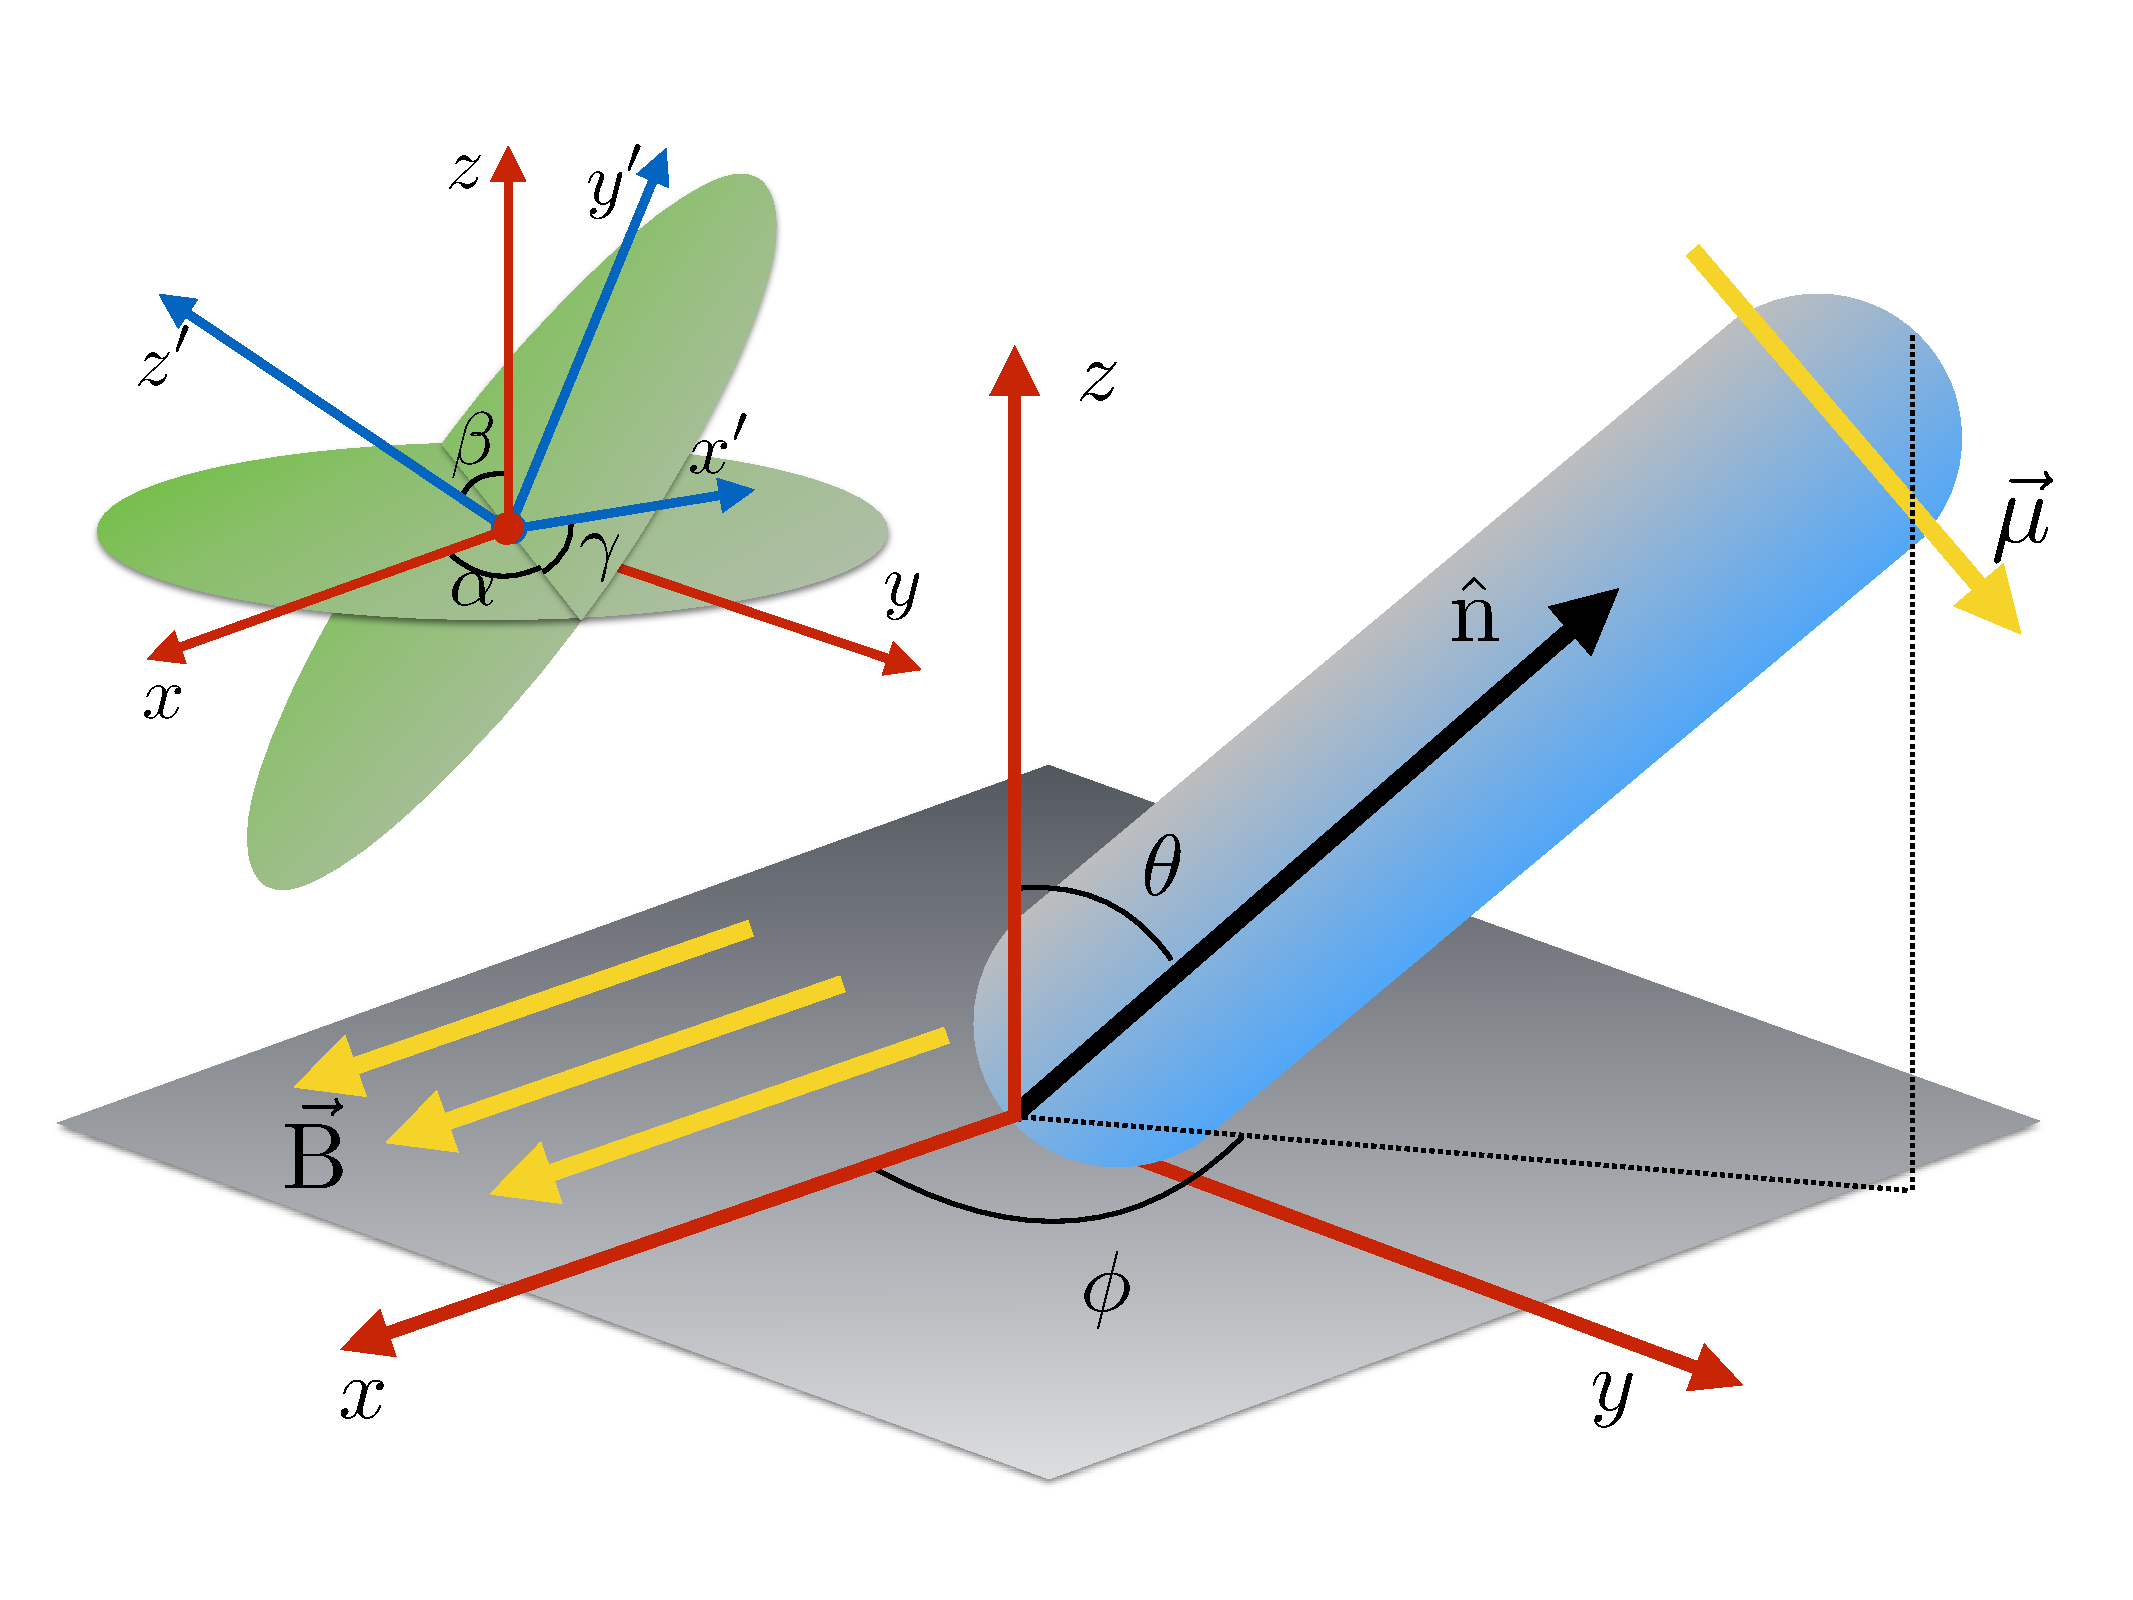
\includegraphics[width=0.8\columnwidth]{figs/geometry.pdf}
	\caption{\footnotesize \emph{Main:} The rod's long axis is spanned by $\hvcrm{n}$ and makes an angle $\theta$ with the $z$-axis. Its projection in the $xy$-plane subtends an angle $\phi$ with the $x$-axis. A perpendicular permanent magnetic moment $\vc{\mu}$ is embedded in one end of the rod and rotates rigidly with it. An external magnetic field $\vcrm{B}$ is applied in the $x$-direction while the gravitational field acts in the $-$ve $z$-direction. \emph{Inset:} Euler angles are useful for describing the fixed-body rotation of the rod, where $\hvcrm{n}=\hvcrm{z}'$, $\vc{\mu}=\mu\hvcrm{x}'$, $\beta=\theta$, and $\alpha=\phi+\frac{\pi}{2}$.\label{fig:geometry}}
\end{figure}



%%%%%%%%%%%%%%%%%%%%%%%%%%%%%%%%%%%%%%%%%%%%%%%%%%%%%%%%%%%%%%%%%%%%
%
%
%
%
%					R E S U L T S 
%
%
%
%%%%%%%%%%%%%%%%%%%%%%%%%%%%%%%%%%%%%%%%%%%%%%%%%%%%%%%%%%%%%%%%%%%%
%\section{Introduction}
\emph{Results.} Due to its large density relative to water, ($\Delta\rho = \rho_r - \rho_w \approx 0.9 \cdot 10^3$ kg m$^{-3}$) a rod undergoes fast sedimentation on the coverslip of the microscope slide and will naturally lie horizontally in the plane ($\theta\lesssim\pi/2$) whilst undergoing rotational Brownian motion in $\phi$ when no external field is present. Thermal deviation far below $\theta=\pi/2$ is exponentially suppressed by gravity. In the presence of an in-plane magnetic field $\vcrm{B}=B \hvcrm{x}$, the magnetic moment $\vc{\mu}$ aligns with $\vcrm{B}$, trapping the rod in the $yz$-plane. The azimuthal angle of the rod fluctuates about either the points $\phi_0=\pm\pi/2$. We make use of the equipartition theorem $ \frac{1}{2}\kk T = \langle -\vc{\mu}\cdot\vcrm{B}\rangle \approx \frac{1}{2}\mu B \langle \Delta\phi^2 \rangle $ to calculate the strength of the moment $\mu$ by measuring the fluctuations $\Delta\phi=\phi-\phi_0$ at varying field strengths at room temperature. The spread of $\Delta\phi$ decreases for larger $B$, and does so in a manner consistent with $\mu(B)$ remaining constant across the full range of fields applied, from which we were able to infer that the rod cap is ferromagnetic. Typically, we measured the strength of the magnetic moment to be approximately $1$-$2\ \kk T $ G$^{-1}$ at room temperature. For the subsequent experiments, we used a rod with a moment strength measured to be $\mu = 1.2\pm0.1\ \kk T$ G$^{-1}$.

The main experimental observation that motivated this study was that confinement of the rods to the $yz$-plane by a magnetic field resulted in the emergence of an apparent bistability between vertical ($\theta \approx 0$) as well as horizontal ($\theta \lesssim \pi/2$) orientations, with thermal fluctuations alone strong enough to excite both states ---in contrast to an energy consuming excitation-relaxation process or a driven process resulting in similar behaviour \cite{Dhar2007}. Importantly, this effect occurs in spite of the fact that the rod gains $\frac{1}{2}\Delta\rho V g (L-d) \approx 3.4 \ \kk T$ of gravitational potential energy at no reduction in magnetic energy $\vc{\mu}\cdot \vcrm{B}$ (as $\vc{\mu}$ is able to remain aligned with the field at all times), which goes against intuition.

\begin{figure}
\centering
\subfloat[][]{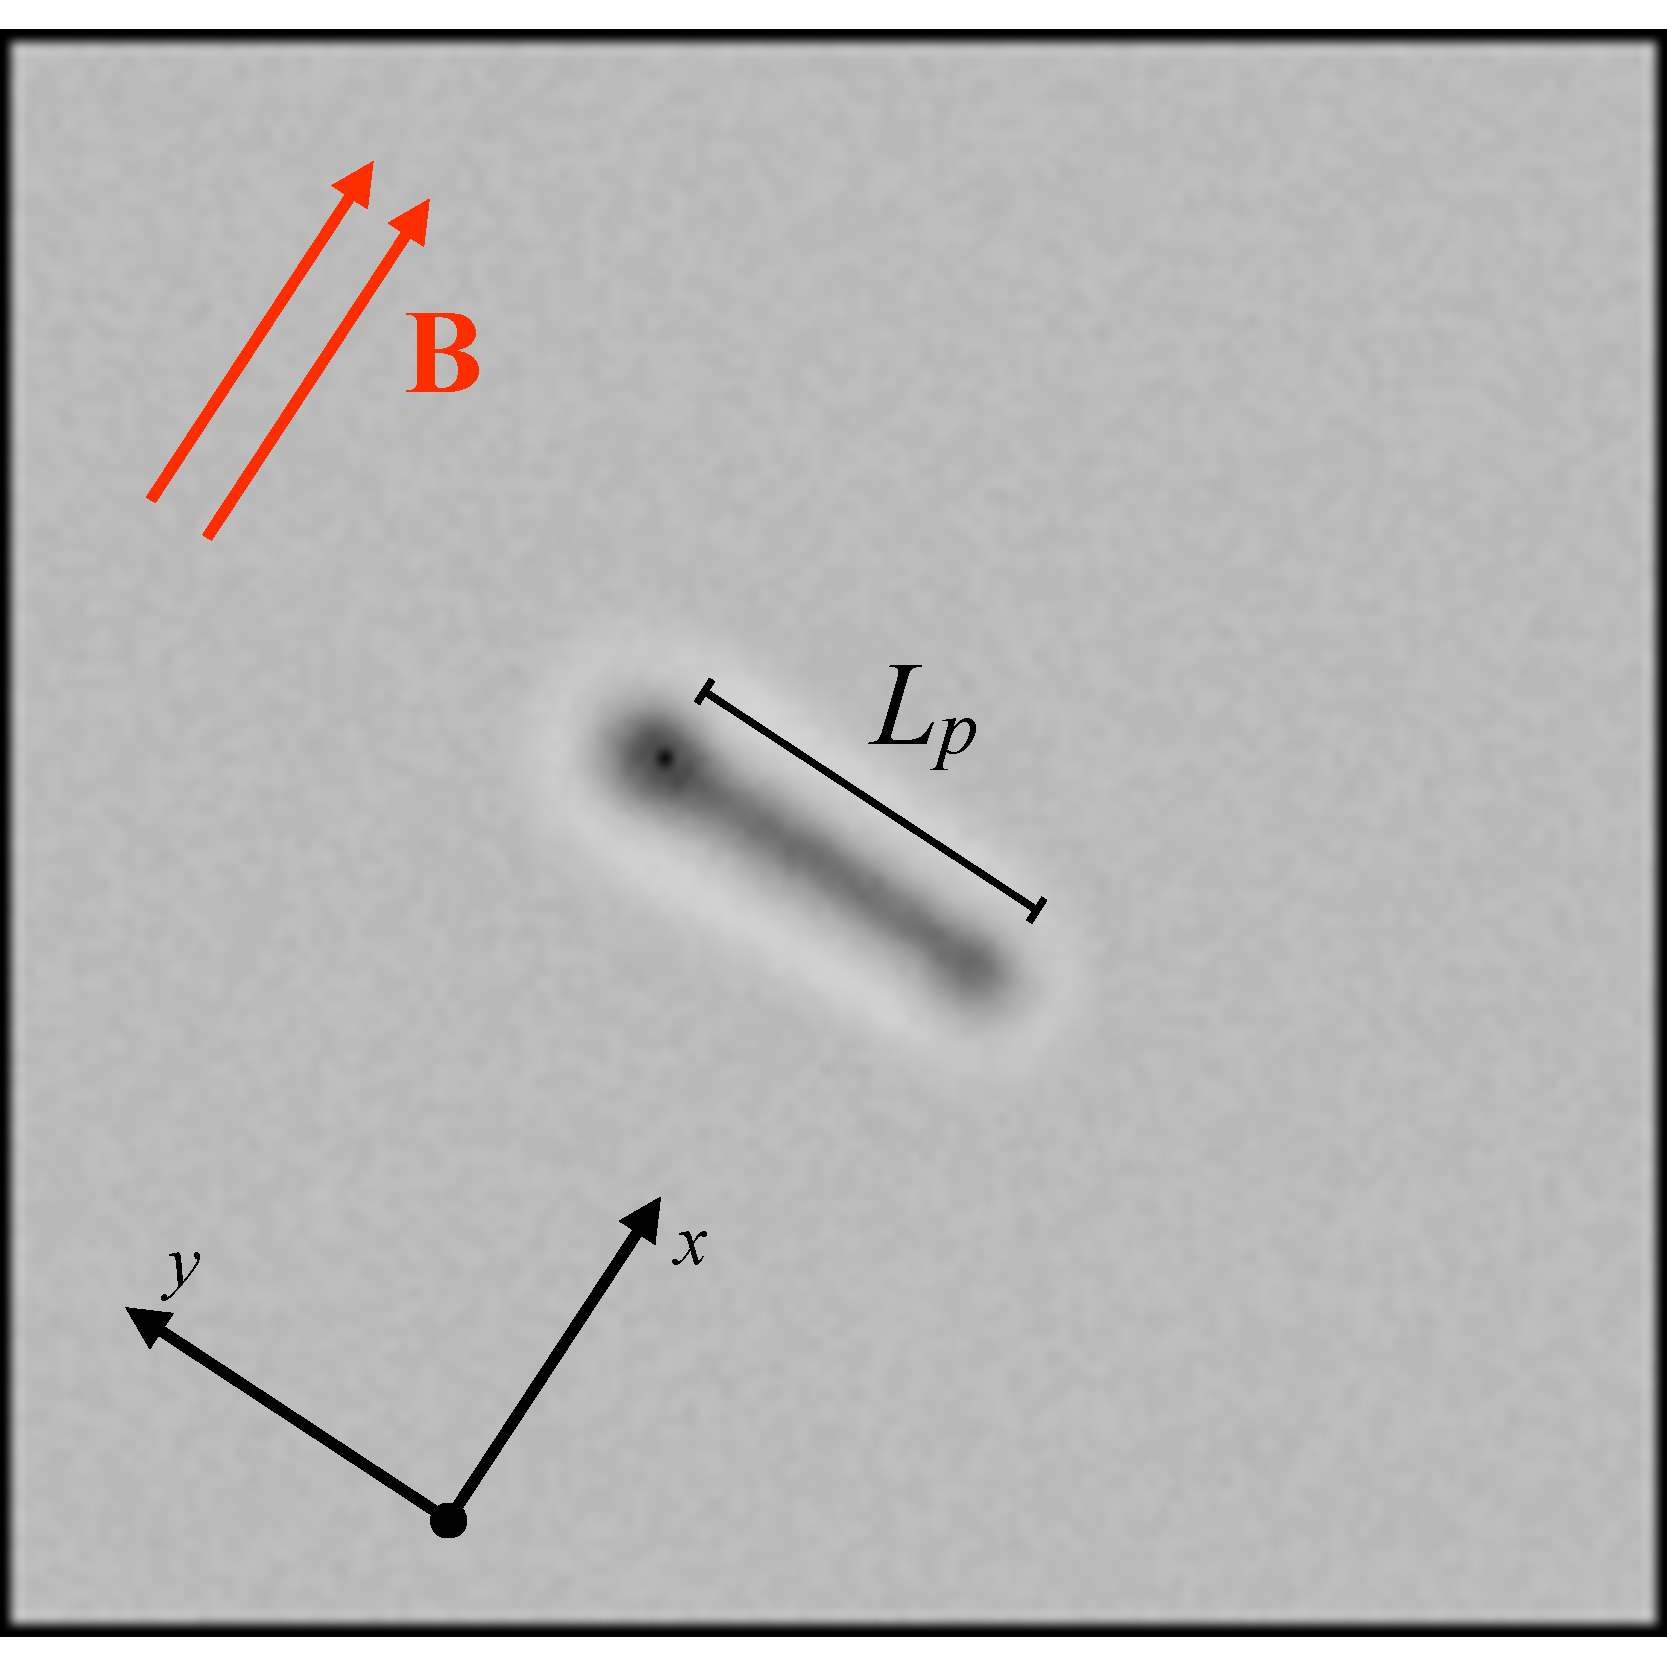
\includegraphics[width=0.3\columnwidth]{figs/Figure3bb}\label{horizontal}}
\subfloat[][]{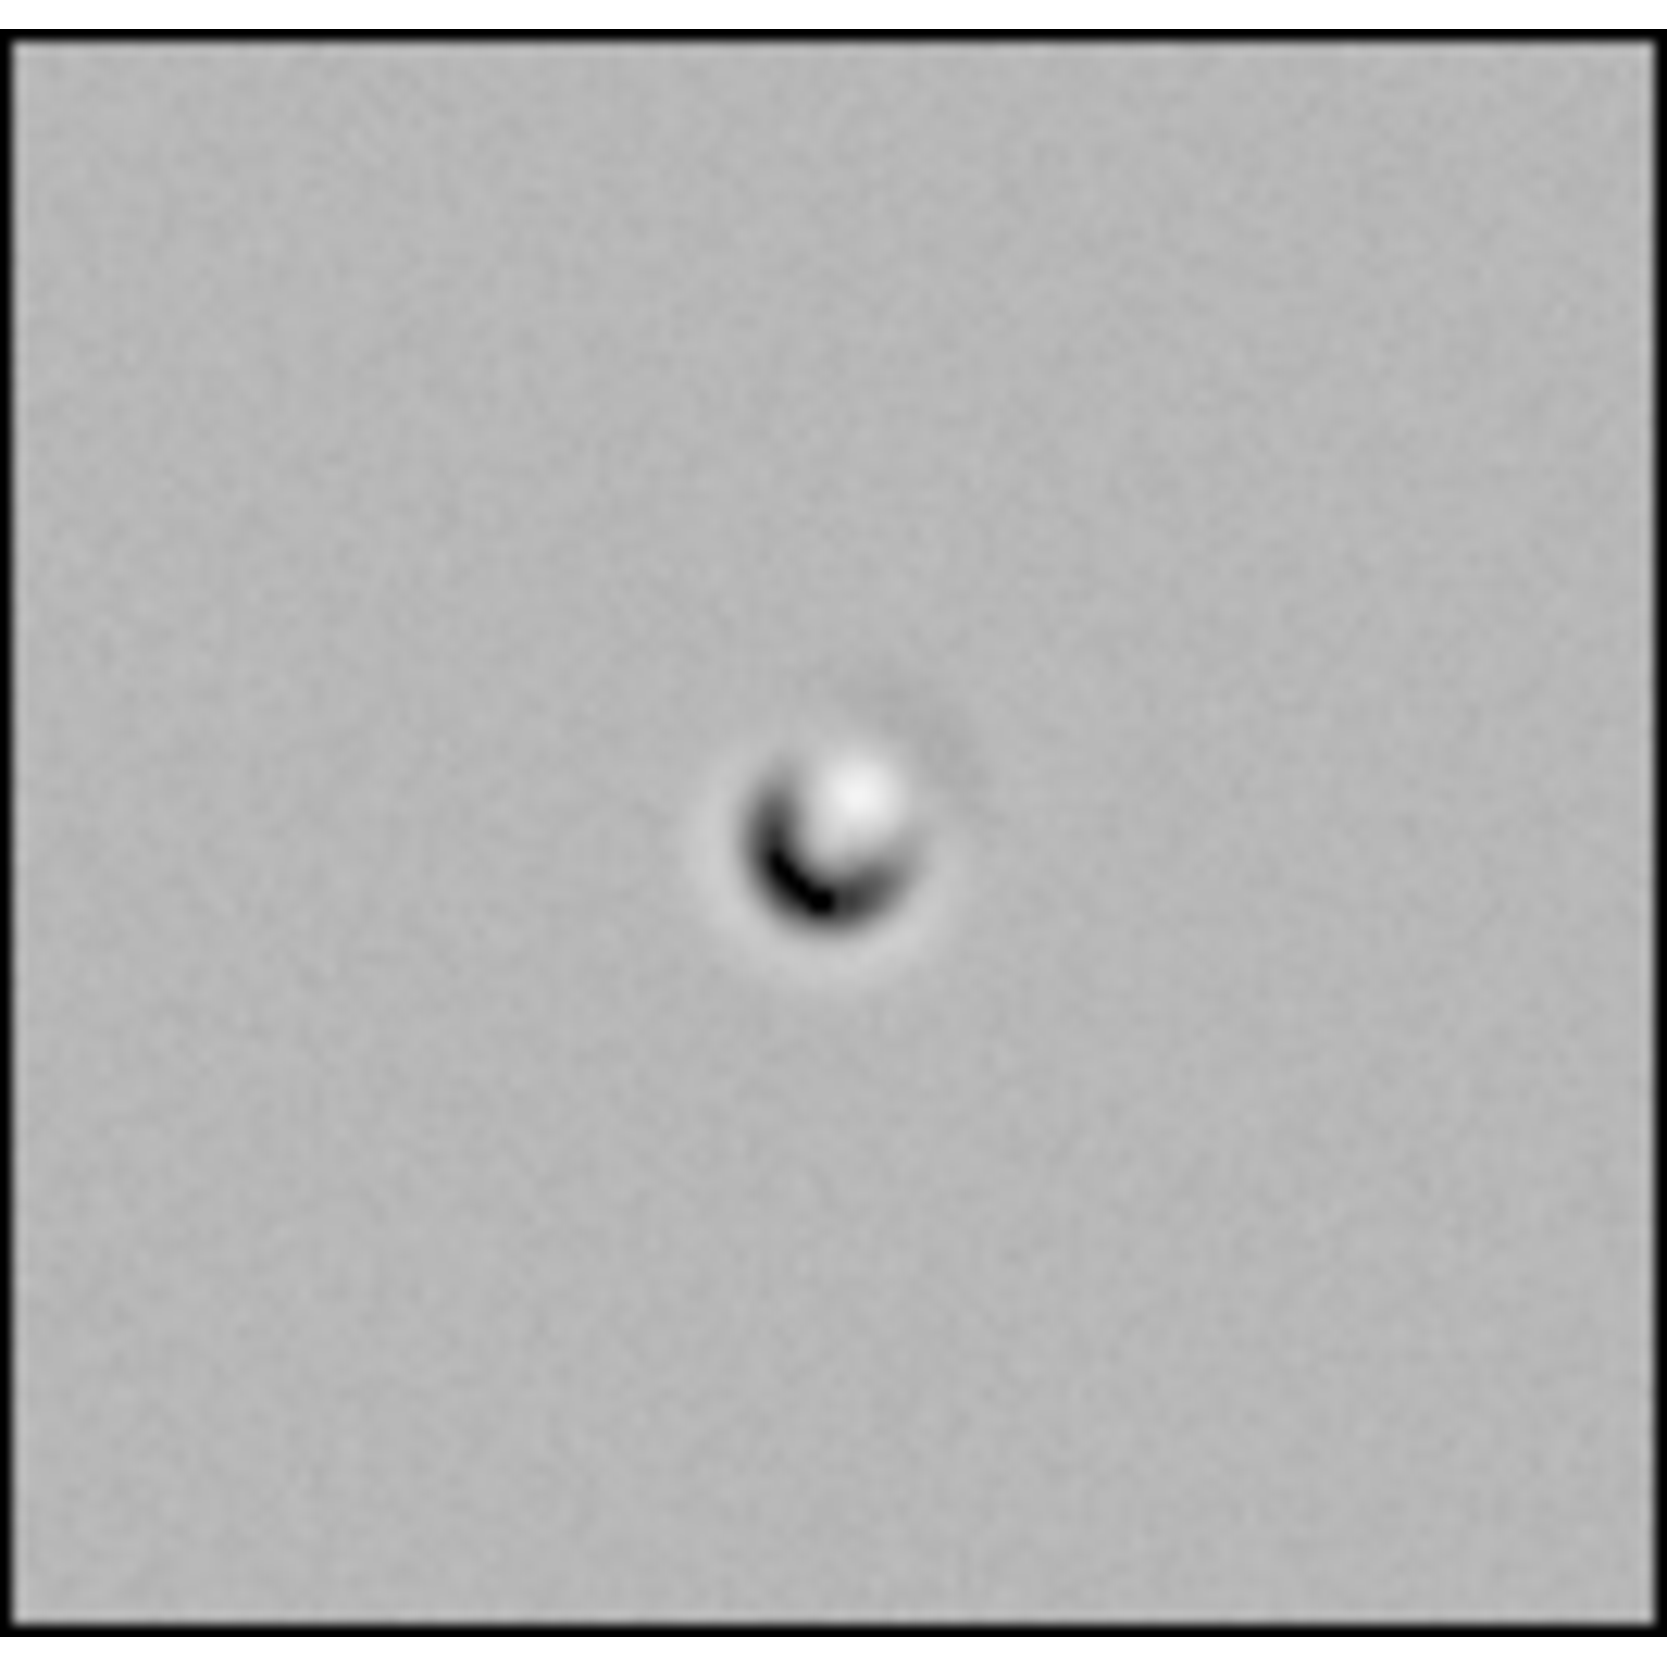
\includegraphics[width=0.3\columnwidth]{figs/Figure3ba}\label{vertical}}
\subfloat[][]{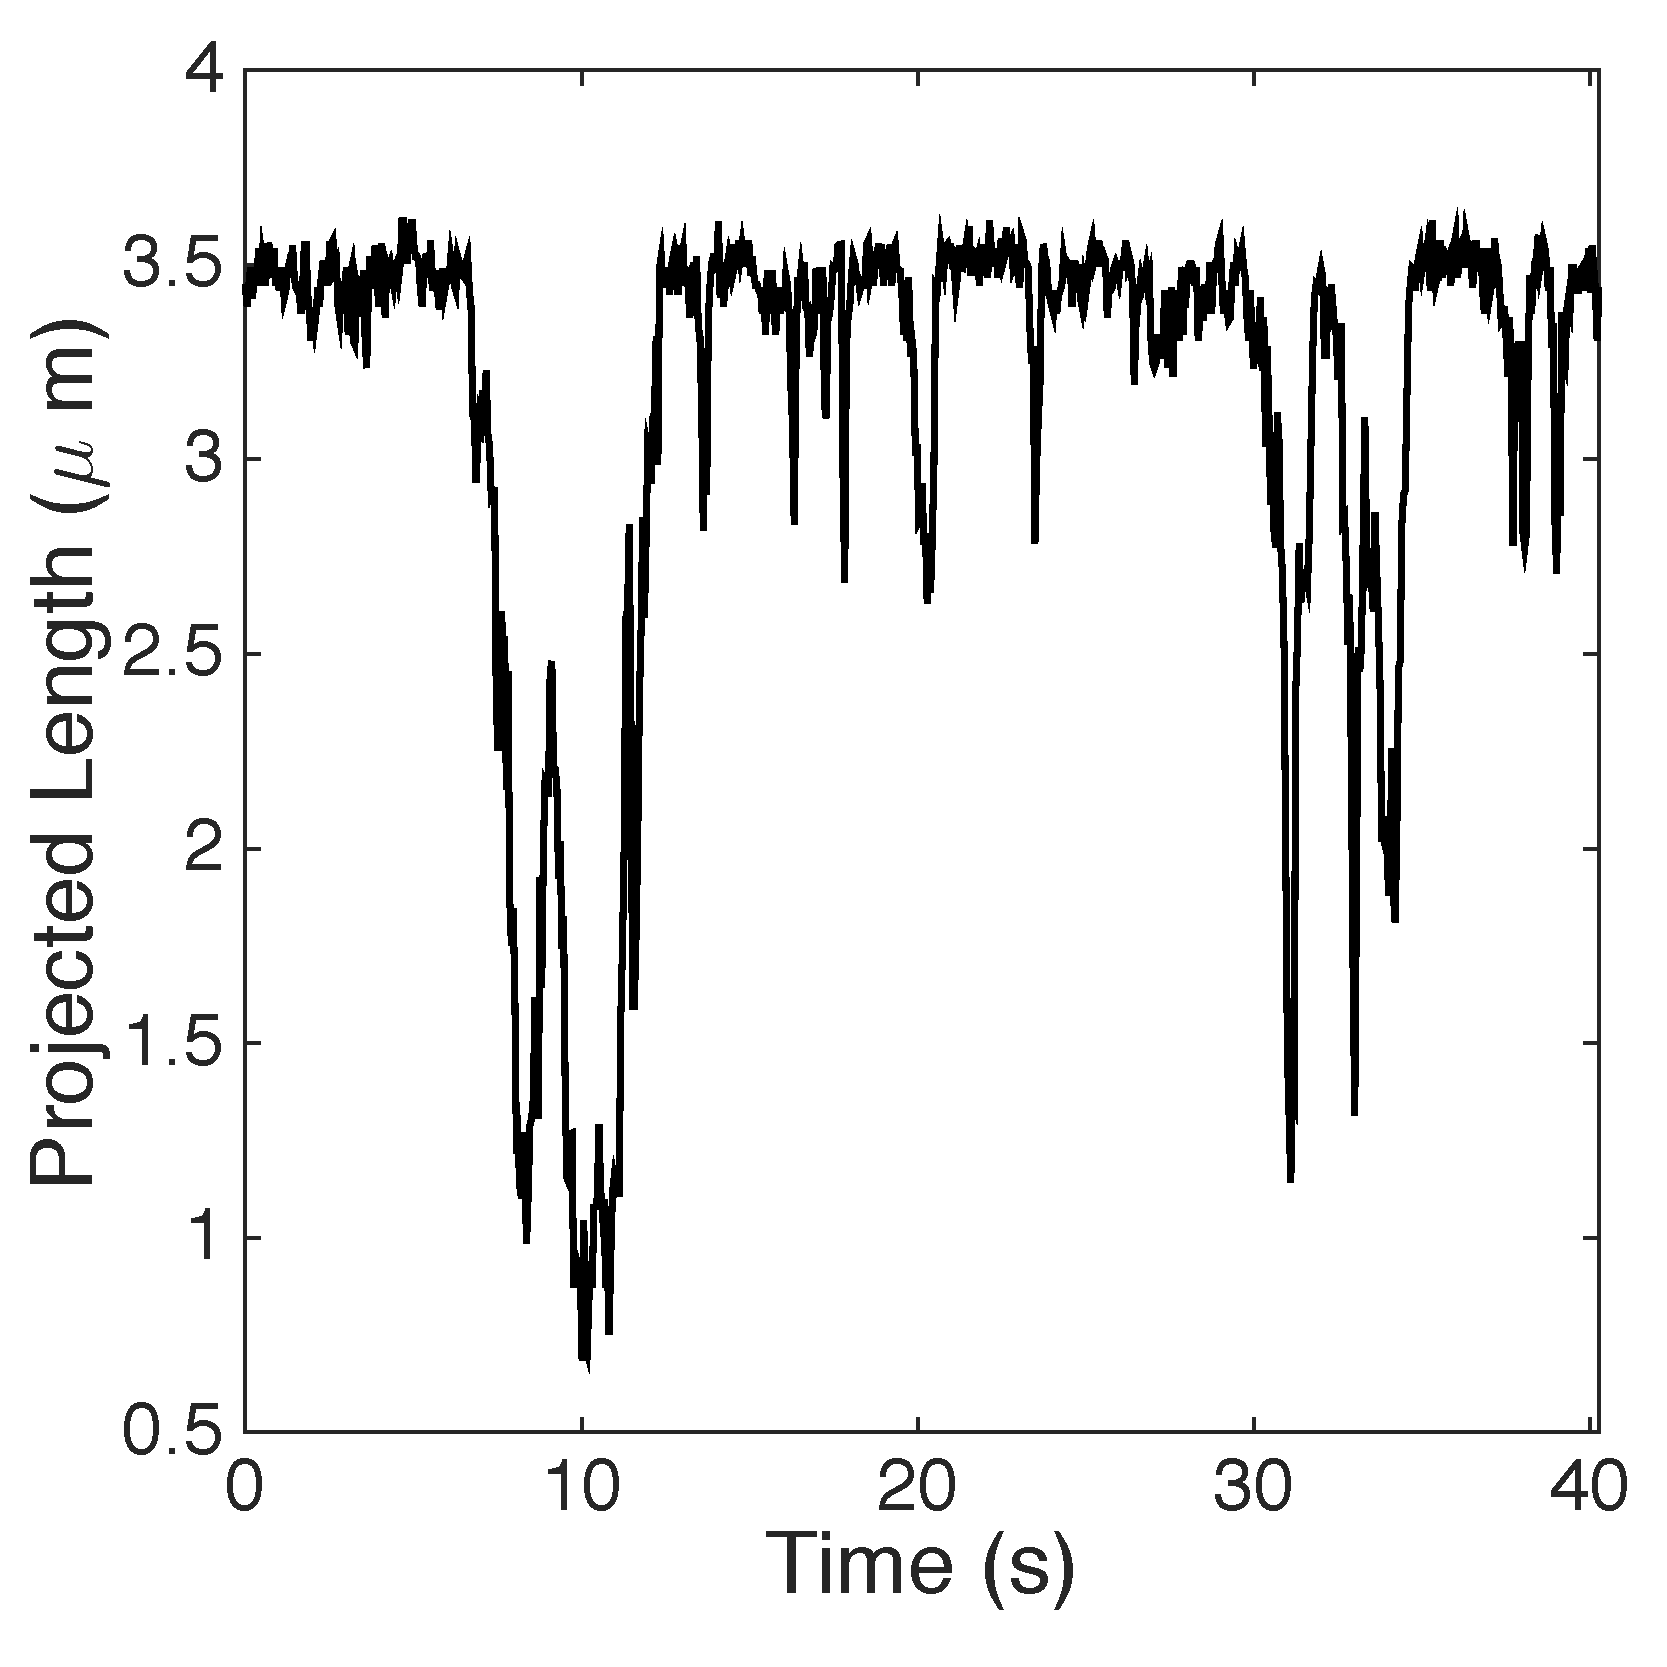
\includegraphics[width=0.3\columnwidth]{figs/Figure3bc}\label{timeseries}} 
    \caption{\footnotesize (a-b) A magnetic field in the $x$-direction is responsible for the trapping of the rod in the $yz$-plane; we observe the rod to hop between two states: (a) horizontally along $\pm y$ with $\theta=\pi/2$, and (b) vertically along $z$, where $\theta=0$. (c) A short segment of projected length $L_p(t)$ demonstrates the `hopping' nature of this behaviour.}
\end{figure}

This dynamic behaviour is best described as a hopping transition between these two states, occurring at random with a characteristic forwards- and backwards-rate and is apparent in real-time video data provided in the Supplementary Information (SI). For illustration, two frames captured at different times are displayed in Figs.\ \ref{horizontal} and \ref{vertical}. By automated analysis of the images, we measured the projected length $L_p(t)$ of the rod in the $xy$-plane at each time, a segment of which is shown in Fig.\ \ref{timeseries}. We also measured the azimuthal angle $\phi(t)$ of the rod in the image plane. Figure \ref{timeseries} shows clearly the hopping behaviour between the horizontal state (large $L_p$) and the vertical state (small $L_p$). We calculated the polar angle using $\theta(t) = \sin^{-1}{[(L_p(t)- d)/(L - d)]}$, where $L=3.5\ (\pm0.01)\ \mu$m and $d=0.65\ (\pm0.01)\ \mu$m were the measured total length and diameter of the rod respectively. Due to the error on these, occasionally a measurement of $L_p(t)$ would fall out of the range $[d, L]$, and would be set to its corresponding bounding value in order for $\theta(t)$ to remain real-positive.
\begin{figure*}
\centering
\subfloat[][]{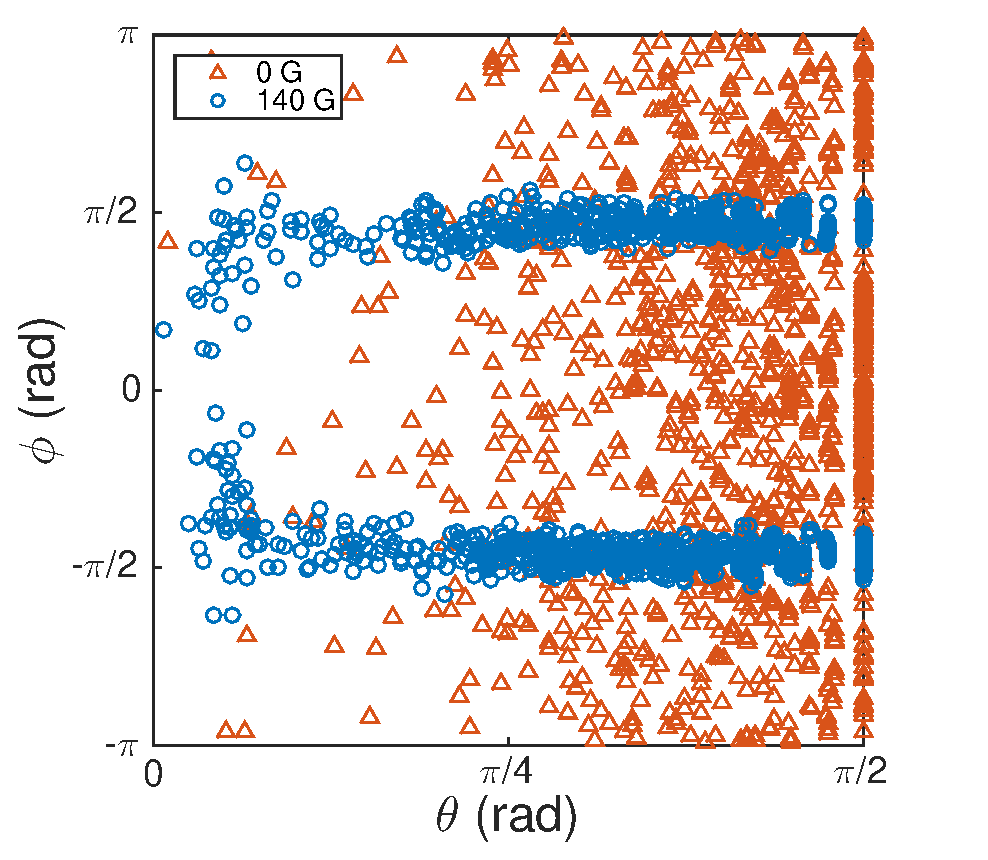
\includegraphics[width=0.5\columnwidth]{figs/Fig3scatter.eps}\label{scatter}}
\subfloat[][]{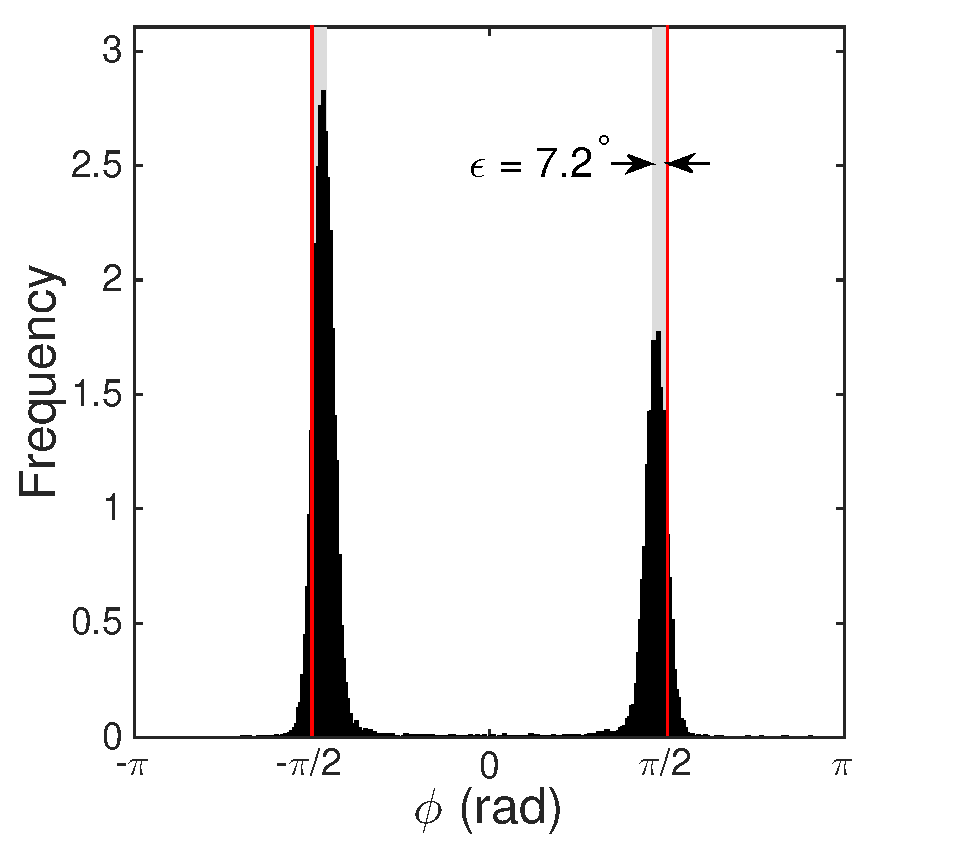
\includegraphics[width=0.5\columnwidth]{figs/Fig3hist.eps}\label{phi_hist}} 
\subfloat[][]{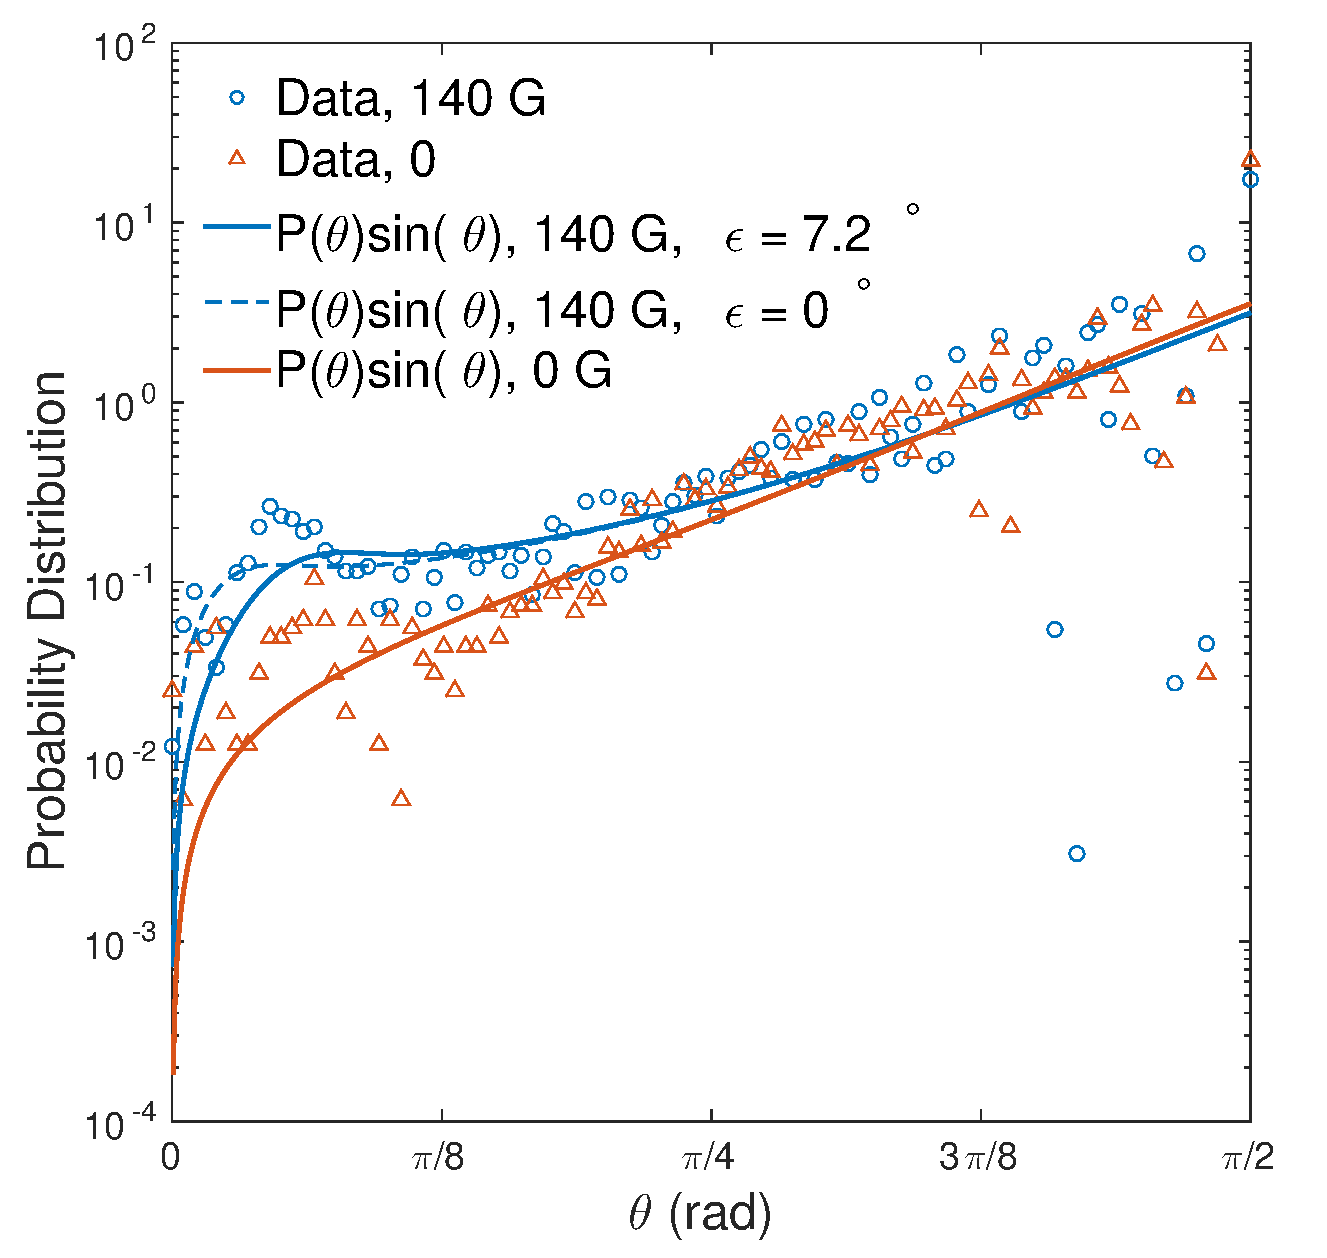
\includegraphics[width=0.5\columnwidth]{figs/Figure3a.eps}\label{Pdata}}
\subfloat[][]{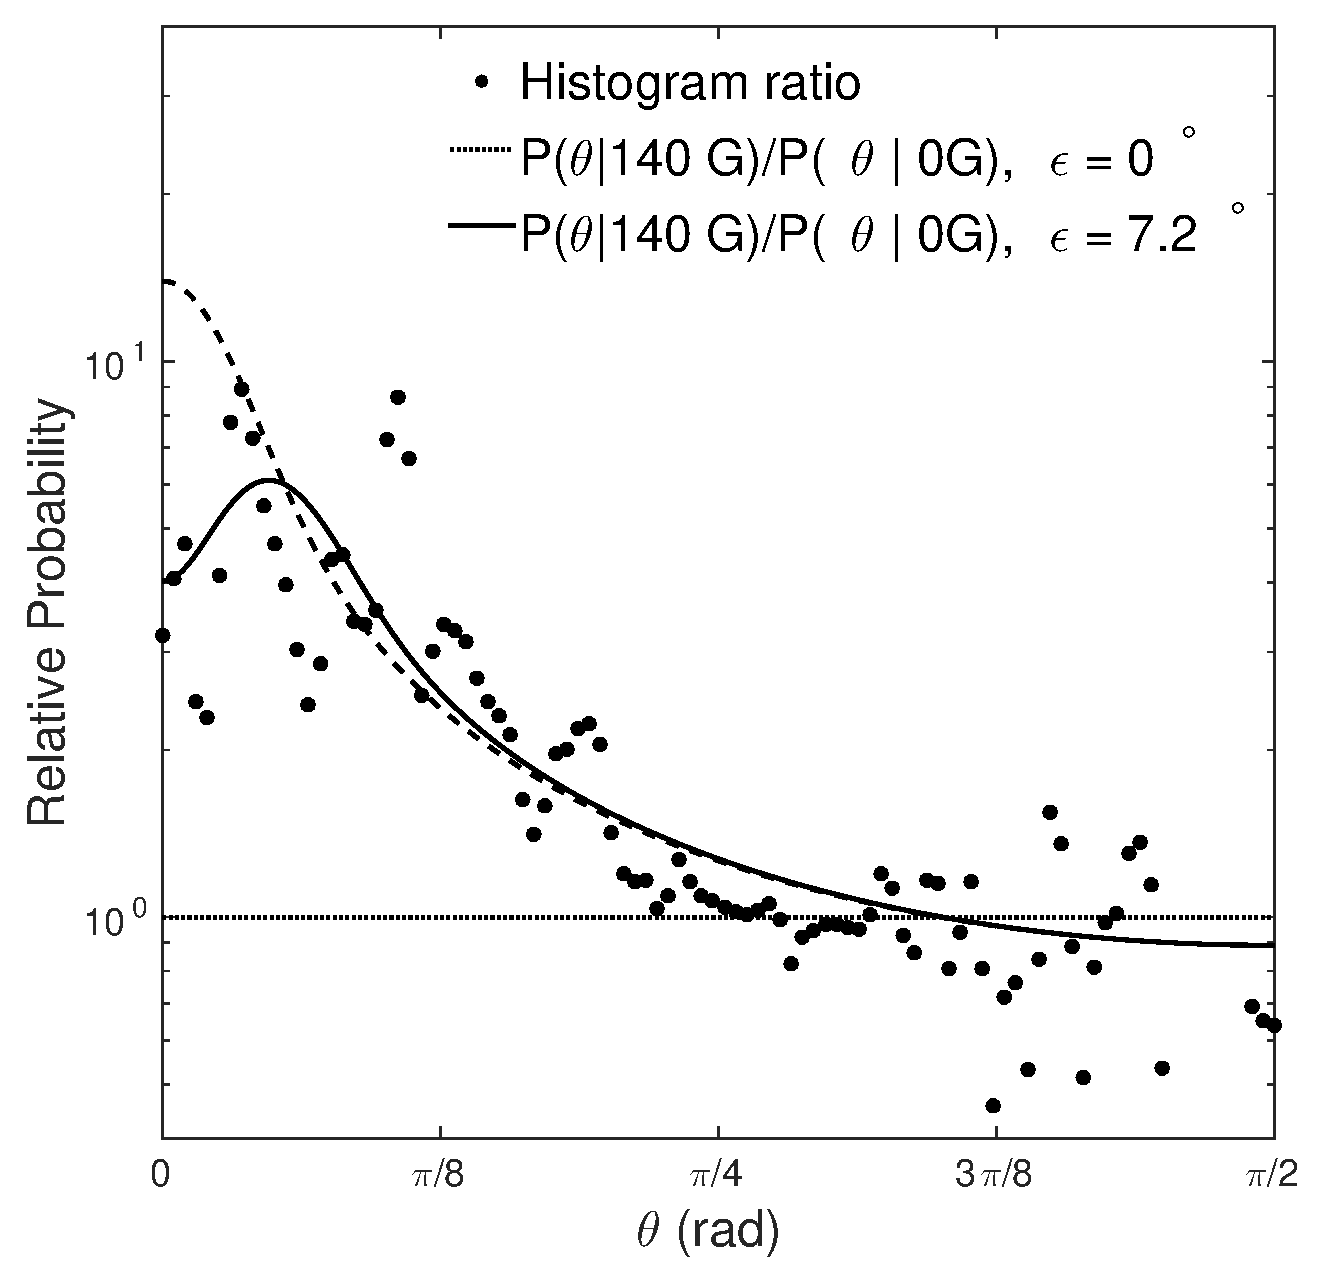
\includegraphics[width=0.5\columnwidth]{figs/Figure3ab.eps}\label{ratio}}
    \caption{\footnotesize (a) Scattered [$\theta(t)$,$\phi(t)$] for no field ($\bigtriangleup$) and $140$ G field ($\bigcirc$) demonstrates the magnetic trapping (for clarity, we display every tenth sequential point). (b) Histogram of $\phi(t)$ for $B=140$ G case enables us us to calculate $\epsilon$ by measuring the offset of the peak from $\pm \pi/2$. (c) Histogram of $\theta(t)$ over 60 minutes shows a markedly increased tendency for vertical states (small $\theta$) to be realised when a magnetic field is present ($\bigcirc$) with respect to a free rod ($\bigtriangleup$). The curves represent absolute probability weightings $P(\theta) \sin(\theta)$ where we have numerically integrated Eq.\ (\ref{corrected}) using independently measured parameters $\mu$, $\epsilon$, $m$, $L$ and $d$. (d) The relative distribution $P(\theta | 140 $G$)/P(\theta | 0 $G$)$ agrees well with the theoretical calculations, showing an $O(10)$ increase in likelihood for small-$\theta$ states due to the magnetic field.}
\end{figure*}



To demonstrate that the presence of a magnetic field is significantly responsible for this effect, we ran two experiments for 60 minutes each at $0$ G and $140$ G field strengths respectively. Figure \ref{scatter} shows the scattered [$\theta(t)$,$\phi(t)$] data and qualitatively demonstrates both the trapping in $\phi$ and the increase in instances of low-$\theta$ measurements in the magnetically confined case. However, a histogram of $\phi(t)$ in the presence of the field (see Fig.\ \ref{phi_hist}) demonstrates a more subtle feature of the data: rather than being trapped exactly along the $y$-axis ($\phi_0=\pm\pi/2$), the mean azimuthal angle of the rod deviated from this by around $\mp0.12$ rad ($= 7.2^\circ$). This is evidence that rather than being precisely within the cross-sectional plane of the rod, $\vc{\mu}$ makes an angle $\epsilon\approx 7.2^\circ$ with it. In the next section, we will theoretically consider both the ideal case that $\vc{\mu}\cdot\hvcrm{n}=0$, as well as an exact description accounting for finite $\epsilon$. Figure \ref{Pdata} contains histograms of $\theta(t)$ in both cases of with and without field and Fig.\ \ref{ratio} clearly shows how the magnetic field accounts for an $\sim O(10)$ increase in relative likelihood of the rod being found in the vertical state. Rather than having a peak at exactly $\theta=0$, note however that due to a finite $\epsilon$, the maximum-likelihood vertical state is offset by about $\sim 0.15$ rad. The curves plotted on top of the data in Figs.\ \ref{Pdata}-\ref{ratio} are discussed in the following section.


%%%%%%%%%%%%%%%%%%%%%%%%%%%%%%%%%%%%%%%%%%%%%%%%%%%%%%%%%%%%%%%%%%%%
%
%
%
%
%					T H E O R E T I C A L   M O D E L 
%
%
%
%%%%%%%%%%%%%%%%%%%%%%%%%%%%%%%%%%%%%%%%%%%%%%%%%%%%%%%%%%%%%%%%%%%%
%\section{Introduction}
\emph{Theoretical Model.} Each state of the rod $(\vm,\vn)$ can be described in terms of the angles $(\phi, \theta, \gamma)$ which relate its fixed-body frame to the laboratory frame. We consider the system as an ensemble of states $(\phi,\theta,\gamma)$ with instantaneous energies $U(\phi,\theta,\gamma)$. We assume that on times much longer than the dynamical timescales, the states form a canonical ensemble. Horizontal translational motion in the $xy$-plane is independent of $U$ so may be factored out of our discussion entirely. We ignore the subtle effects of vertical translational freedom, assuming that the rod is always in contact with the substrate. Under these assumptions, the total energy of the system in a given state can be written as a sum of magnetic and gravitational terms: $U = -\vm \cdot\vB + \frac{m^*l}{2} \vn \cdot \vcrm{g}$, where $m^*=\Delta\rho V$ is the effective mass of the rod, and $l=L-d$ is the length of the cylindrical section. We evaluate each term in the rod's fixed body frame $(x',y',z')$, where $\vc{\mu}' :=\mu(\cos\epsilon,0,\sin\epsilon)$ and $\hvcrm{n}' :=(0,0,1)$. For an ideal rod, $\epsilon=0$ means the magnetic moment is purely orthogonal to the axis of the rod. The external fields in this frame are thus given by solid body rotations: $\vcrm{B}' = \vcrm{R}(\phi,\theta,\gamma)\cdot ( B \hvcrm{x})$, and $\vcrm{g}'= \vcrm{R}(\phi,\theta,\gamma)\cdot ( -g \hvcrm{z})$, where $\vcrm{R}(\phi,\theta,\gamma)$ is the rotation matrix describing the laboratory- to rod-frame transformation. It can be shown (see SI) that

\begin{eqnarray}
U(\phi,\theta,\gamma) & = & -\mu B \Big( \cos\epsilon [\ccc\ssp + \cct\ccp\ssc] \nonumber \\
& + & \sin\epsilon \cos\phi\sin\theta \Big) + \frac{m^*gl}{2} \cct.
\end{eqnarray}

The equilibrium distribution of the rod is the Boltzmann distribution $P(\theta, \phi, \gamma)  =  \frac{1}{Z} \ee^{ -U(\phi, \theta, \gamma)/\kk T }$ where the partition function is given by:

\begin{eqnarray}
Z  =  \int_0^{\frac{\pi}{2}} \sst\ \dd\theta \iint_{-\pi}^{\pi}\ \dd\phi\ \dd\gamma \ \ee^{ -U(\phi, \theta, \gamma)/\kk T }.
\end{eqnarray}

As $\gamma$ is not measured by experiment we wish to first find the marginal distribution $P(\theta,\phi)$ by integrating out the $\gamma$ dependence. To simplify the notation, we introduce the relative strength of the gravitational energy $a=m^*gl/2 \kk T$ and magnetic energy $b=\mu B/\kk T$. The integral may be carried out explicitly, giving:


\begin{eqnarray}\label{corrected}
P(\theta,\phi)  & = & \frac{\ee^{-a\cos\theta}}{Z} \Big\{ I_0\Big( b\cos\epsilon\sqrt{1-\cos^2\phi\sin^2\theta} \Big) \nonumber\\
& \times &  \ee^{-b \sin\epsilon \cos\phi\sin\theta}\Big\} \label{P_corrected}
\end{eqnarray}

where $I_0(x)$ is the modified Bessel function of the first kind. This distribution contains no adjustable parameters as $a=3.4$, $b=156$, and $\epsilon=7.2^\circ$ are all independently measurable for a given rod.


\begin{figure*}
\centering
\subfloat[][]{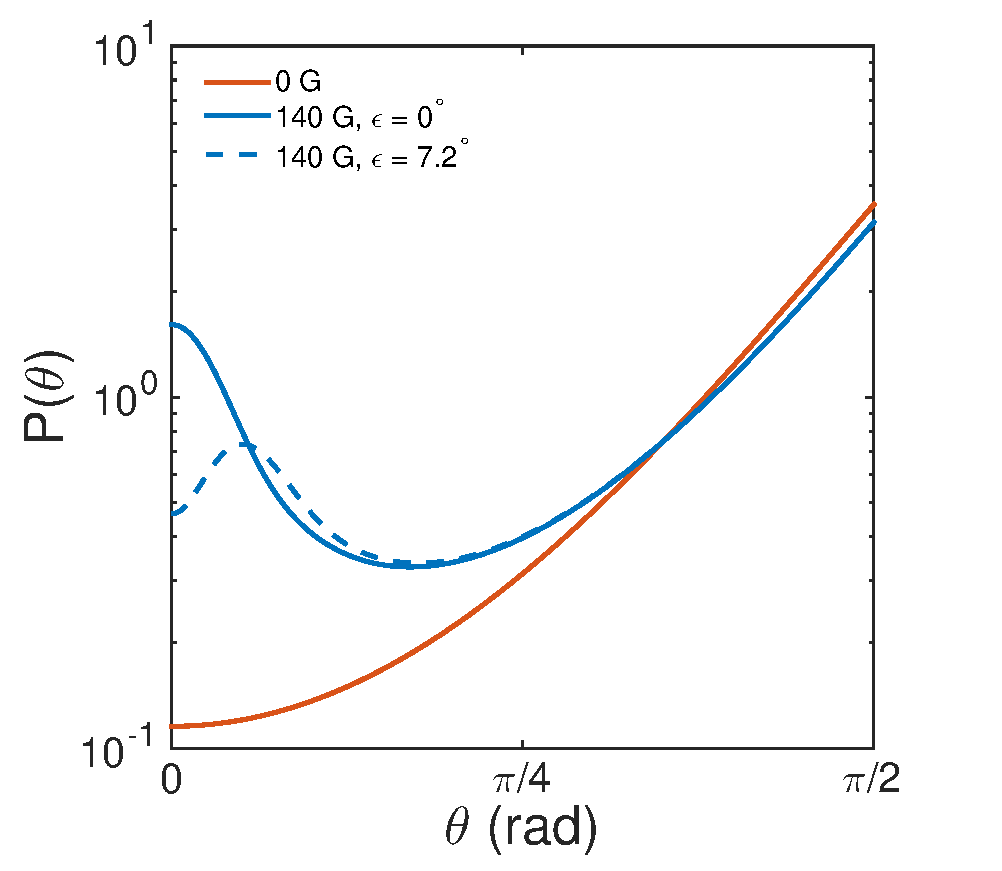
\includegraphics[width=0.4\columnwidth]{figs/Figure4.eps}\label{theorya}}
\subfloat[][]{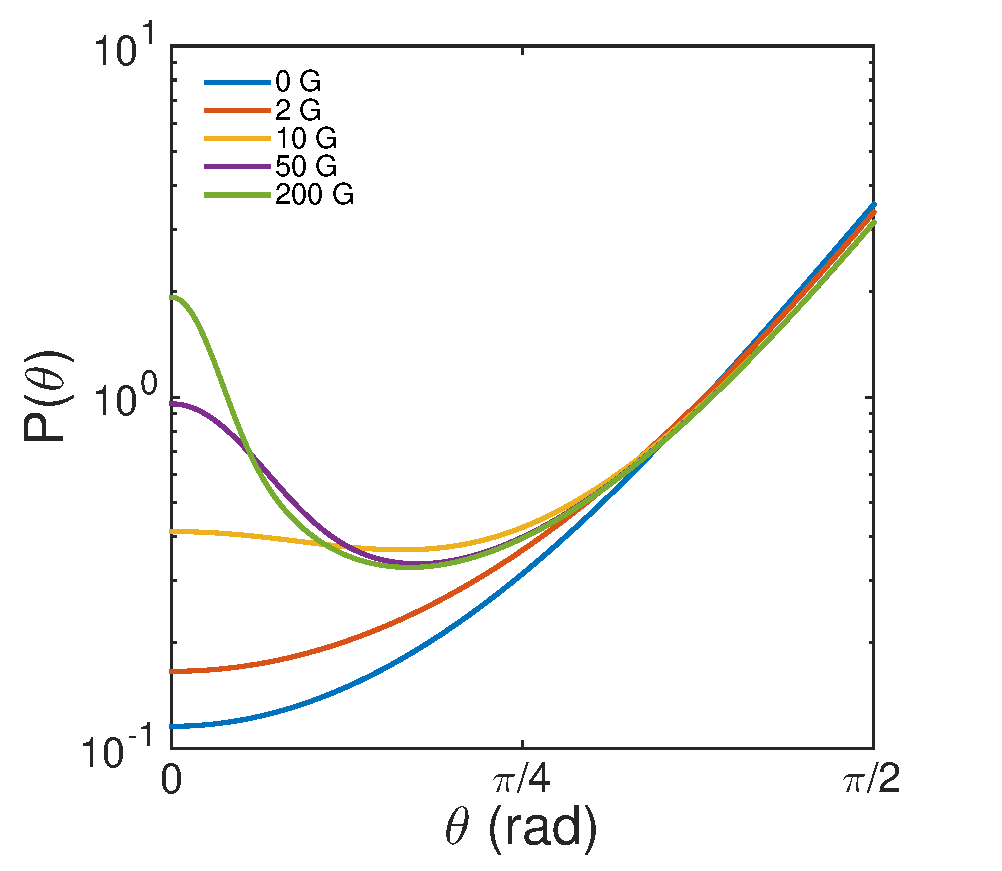
\includegraphics[width=0.4\columnwidth]{figs/Figure4b.eps}\label{theoryb}}
\subfloat[][]{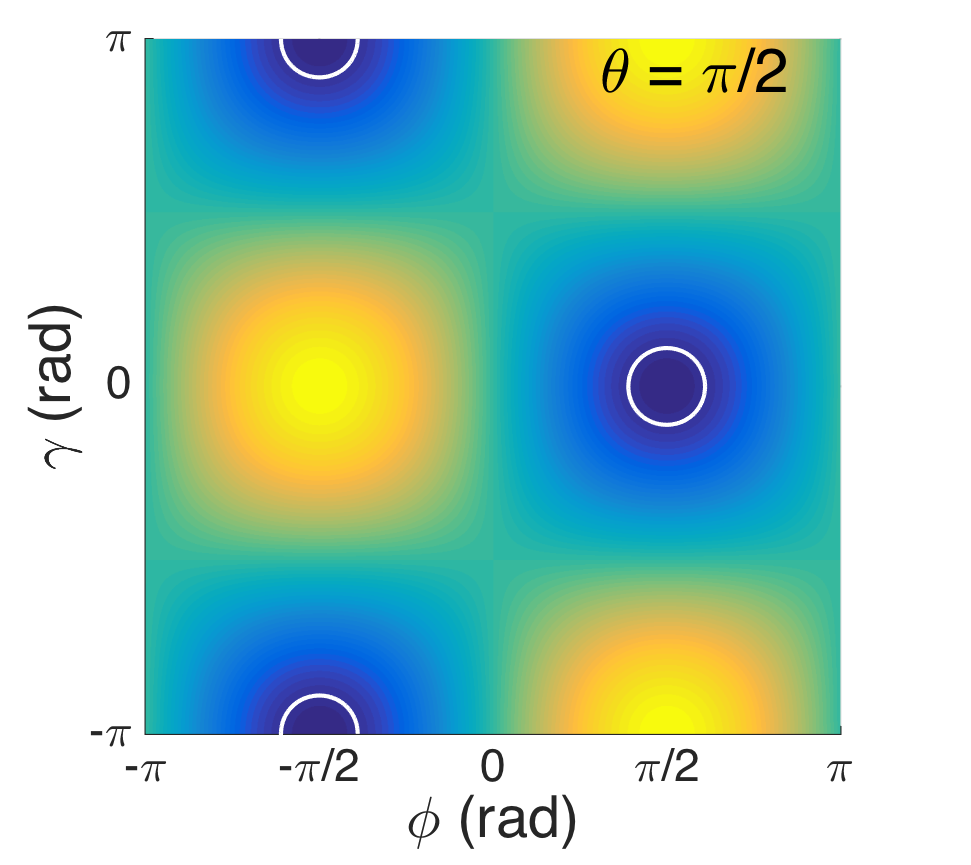
\includegraphics[width=0.4\columnwidth]{figs/Figure5a.eps}\label{phasea}}
\subfloat[][]{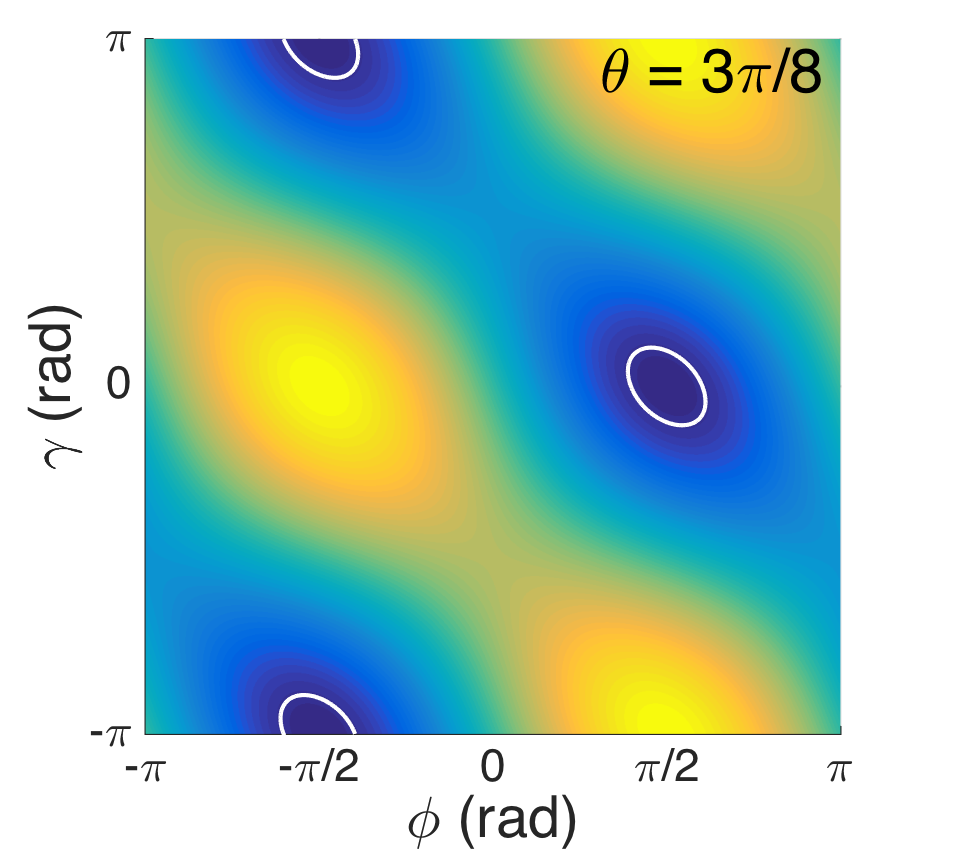
\includegraphics[width=0.4\columnwidth]{figs/Figure5b.eps}\label{phaseb}}
\subfloat[][]{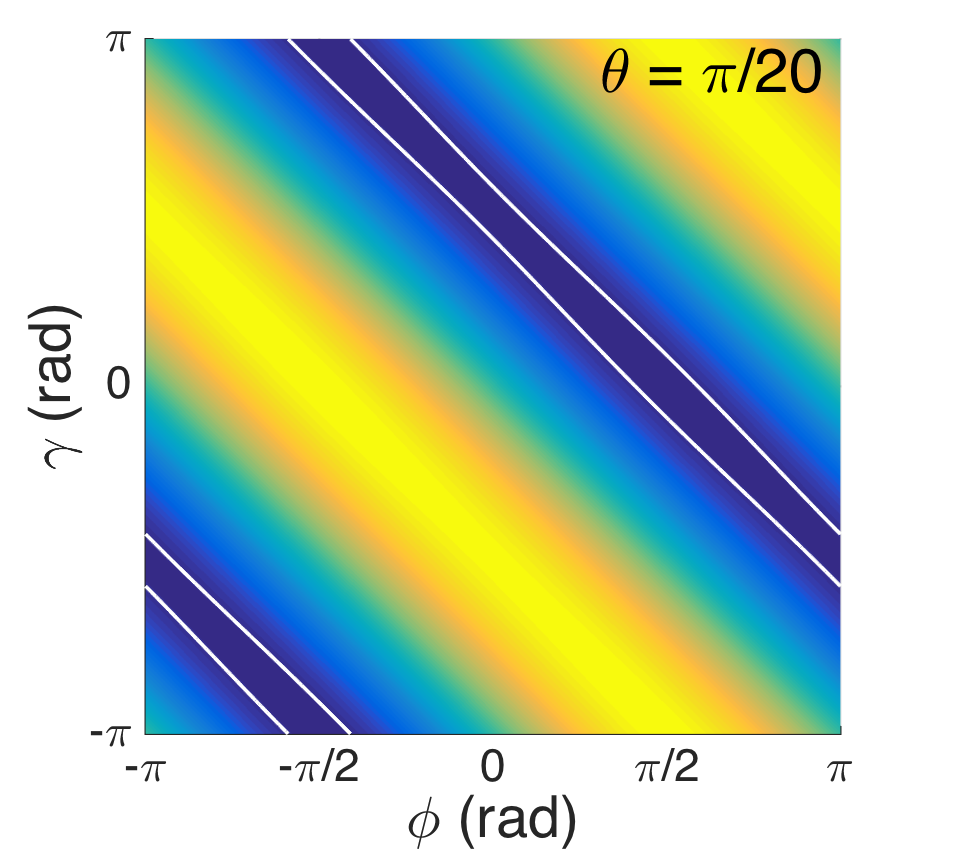
\includegraphics[width=0.4\columnwidth]{figs/Figure5c.eps}\label{phasec}}
    \caption{\footnotesize (a) Probability density function for a rod with $\mu=1.2\ \kk T$ G$^{-1}$ in $140$ G (blue) and $0$ G (red) fields shows an emergent bistability between vertical and horizontal states brought on by the external field for an ideal rod (---) and one where $\vc{\mu}$ is offset from the cross-sectional plane by $\epsilon=7.2^\circ$ (- -). (b) Same as (a) but for varying magnetic fields. (c-e) The energy $U(\phi,\theta=\Theta,\gamma)$ for three polar angles $\Theta=\frac{\pi}{2},\frac{3\pi}{8},\frac{\pi}{20}$ shows the loss of a degree of freedom. When the rod is lying flat, $\phi$ and $\gamma$ are independently constrained, but when vertical only the compound angle $\phi+\gamma$ is constrained. This results in the entropic favouring of vertical states compared to intermediate states despite the gravitational cost of standing up. \label{theory}}
\end{figure*}

We numerically integrated Eq.\ (\ref{P_corrected}) with respect to $\phi$, and plot the resulting distribution $P(\theta)$ in Fig.\ \ref{theorya} with the same parameters as above but for both $\epsilon=0.0^\circ,7.2^\circ$. In Fig.\ \ref{theoryb}, we calculate $P(\theta| B)$ for many values of $B$ to show how the system transitions from monostability to bistability. This transition occurs at around $b > O(10)$ (i.e.\ when $b > a$), and becomes strong (i.e.\ $P(\pi/2)/P(0) \approx O(1)$) at around $b=O(100)$. The overall effect of applying a large field is to encourage the population of low-$\theta$ states that are otherwise gravitationally suppressed, revealing a minimum at $\theta_{\text{min}}\ne 0$. Considering the quantity -$\ln P(\theta)$, we interpret there as being an effective barrier separating two bistable states. We identify this as an entropic barrier because it does not come from the potential energy which, while keeping $\vc{\mu}\cdot\vcrm{B}$ minimised (with the angles $\phi=\pi/2,\gamma=0$ trapped by the field), is a monotonic function of $\theta$.


To compare the $P(\theta)$ with experiment, we plot the absolute probability $P(\theta)\sin(\theta)$ on top of the histogram of $\theta(t)$. Both are in good agreement and the $140$ G data shows a clear peak at $\theta=0.15$ rad. There appears to be a slight systematic excess in the low-$\theta$ region of the data, however this is factored out when we plot the relative likelihood $P(\theta | 140$ G$)/P(\theta | 0$ G$)$ on top of the corresponding ratio of the histograms. 




 
 %%%%%%%%%%%%%%%%%%%%%%%%%%%%%%%%%%%%%%%%%%%%%%%%%%%%%%%%%%%%%%%%%%%%
%
%
%
%
%					D I S C U S S I O N 
%
%
%
%%%%%%%%%%%%%%%%%%%%%%%%%%%%%%%%%%%%%%%%%%%%%%%%%%%%%%%%%%%%%%%%%%%%
%\section{Introduction}
\emph{Discussion.} We wish to interpret the marginal distribution $P(\theta)$. If we consider a generalised potential $U(q_1,q_2)$ then in units where $\kk T=1$ we have that:

\begin{equation}\label{log-marginal}
\ln{P(q_1)} = \ln\Big[ \int_{Q_2} \dd q_2\ \ee^{-U(q_1,q_2)} \Big] + F,
\end{equation}with $F=-\ln Z$. If $q_1$ and $q_2$ are independent (as in most familiar cases, e.g.\ harmonic potentials $U(x,y)= k_x x^2 + k_y y^2$) then this reduces to $\ln P(q_1)  = -U_1(q_1) + F_1$ and so $\ln P(q_1)$ is proportional to the potential energy landscape $U_1(q_1)$ up to an additive constant. However when this is not the case ---for instance in cases like ours where rotational potentials couple the coordinates to one another--- then Eq.\ (\ref{log-marginal}) is not so readily interpreted as a thermodynamic quantity. However, if we take the negative partial derivative with respect to $q_1$, we get:
\begin{eqnarray}
-\kk T\frac{\partial }{\partial q_1} \ln{P(q_1)} & = & \frac{\int_{Q_2} \dd q_2 \ \frac{\partial U(q_1,q_2)}{\partial q_1} \ee^{-U(q_1,q_2)} }{\int_{Q_2} \dd q_2 \  \ee^{-U(q_1,q_2)}}\nonumber \\ 
& = & \Big\langle \frac{\partial U(q_1,q_2)}{\partial q_1} \Big\rangle_{q_2}.
\end{eqnarray}

The right-hand-side of this has the form of an effective force which we identify as an entropic force. Now for a rod at an angle $\theta=\Theta$:

\begin{equation} \label{entropicforce}
-\kk T\frac{\partial }{\partial \theta}\Big|_{\theta=\Theta} \ln{P(\theta)}  = \Big\langle \frac{\partial U(\theta,\phi,\gamma)}{\partial \theta}\Big|_{\theta=\Theta} \Big\rangle_{\phi,\gamma}
\end{equation}where the average is taken over the angles $\phi,\gamma$.

This allows us to understand why our intuition fails. Naively, one would think that for a rod that has found its global energy minimum where $\vc{\mu}$ is aligned along $\vcrm{B}$ while lying flat, the fact that any change in $\theta$ acts only to increase the potential energy ---while leaving $\vc{\mu}\cdot\vcrm{B}$ unchanged--- means such a change should be suppressed exponentially. However, Eq.\ (\ref{entropicforce}) tells us that we we must take into account the cost of thermal excursions away from this extremal trajectory. As can be seen from Figs.\ \ref{phasea}-\ref{phasec}, decreasing $\theta$ opens up a larger region of phase-space available to the rod. When the rod is lying flat, $\phi$ and $\gamma$ are independently and tightly constrained such that the rod is confined to a well shown in Fig. \ref{phasea}. In the opposite limit $\theta\rightarrow0$, only the compound angle $\phi+\gamma$ is defined, opening up a much larger configuration-space available to the rod. Between Figs.\ \ref{phasea} and \ref{phaseb} ($\theta=\pi/2\rightarrow 3\pi/8$), the gravitational energy increases substantially so $P(\theta)$ decays as $\theta$ is decreased. However, between Figs.\ \ref{phaseb} and \ref{phasec} ($\theta=3\pi/8\rightarrow\pi/20$) there is a smaller yet nevertheless positive gravitational cost, but the coinciding gain in available configuration-space is large enough to compensate for this, hence the hopping that we observed experimentally is a true entropy-driven process. In classical mechanics, this loss of one degree of freedom is associated with gimbal lock: a phenomenon where a mechanical instrument controlled by Euler-like rotations irreversibly loses a degree of freedom when two axes coincide. Unlike this however, the rod is not controlled by Euler-angle rotations; rather it is controlled by frame independent external forces which result from a potential energy which suffers a loss of degree of freedom when the rod aligns perpendicular to the plane of sedimentation. While in mechanical systems, gimbal lock results in a reduction of control of the system, for a thermal system, an analogue of gimbal lock in the potential energy function results in an entropic gain of explorable phase space.

%%%%%%%%%%%%%%%%%%%%%%%%%%%%%%%%%%%%%%%%%%%%%%%%%%%%%%%%%%%%%%%%%%%%
%
%
%
%
%					C O N C L U S I O N S
%
%
%
%%%%%%%%%%%%%%%%%%%%%%%%%%%%%%%%%%%%%%%%%%%%%%%%%%%%%%%%%%%%%%%%%%%%
%\section{Introduction}
\emph{Conclusions.} Measuring the polar angle of a rod is challenging due to optical aberrations which occur when the rod vertically extends beyond the focal plane. Our assumption that $L_p=(L-d)\sin\theta + d$ is therefore inexact in the low-$\theta$ limit. Nevertheless, we have still succeeded in resolving the increased tendency for the rod to hop between states under a magnetic field both in the time series and histogram of $\theta(t)$ and the supporting theory makes a prediction that matches the data well. Even if some systematic error is present in the low-$\theta$ region, this is factored out by considering the relative likelihood ratio, which agrees well with $P(\theta|140 \text{G})/P(\theta|0 \text{G})$ which was calculated.
%Furthermore, both the theoretically predicted likelihood ratio $P(\theta|140 \text{G})/P(\theta|0 \text{G})$ and the same ratio from the data do show good agreement, suggesting that the theory makes a valid explanation of the differential effect of applying the magnetic field.

Our explanation of this effect highlights some subtle but fundamental physics. The rod's broken axial symmetry due to the perpendicular moment means that when coupled to perpendicular fields ($\vcrm{g}$ and $\vcrm{B}$), the energy is necessarily parameterised by three angles. As such it will suffer the inevitable loss of a degree of freedom when two axes of rotation coincide. This loss results in a reduction in the degree of confinement of the rod and so becomes entropically favourable despite coming at a necessary and substantial energy cost.  Indeed any particle with an energy possessing no orientational continuous symmetry may be susceptible to this kind of strong entropic effect under the correct temperature conditions.
  
Y.G.\ and A.K.B.\ contributed equally to this work.

%For a rod pivoting about one of its ends, it feels a gravitational torque $\vc{\tau}_g = \frac{m^* L}{2} \hvcrm{n}\times\vcrm{g}$, where $\vcrm{g} = -g\hvcrm{z}$ is the gravitational acceleration. In the presence of an external magnetic field, an additional torque $\vc{\tau}_B = \hvc{\mu}\times\vcrm{B}$ is felt. At $T=290$ K, the characteristic strengths of these torques are $|\vc{\tau}_g| \sim 6 \kk$T, and $|\vc{\tau}_B| \sim\ $0-250$\ \kk$T (for fields in the range of $B=\ $0-120 G)

%\emph{Distribution}


%\section{}
% Put \label in argument of \section for cross-referencing
%\section{\label{}}
%\subsection{}
%\subsubsection{}

% If in two-column mode, this environment will change to single-column
% format so that long equations can be displayed. Use
% sparingly.
%\begin{widetext}
% put long equation here
%\end{widetext}

% figures should be put into the text as floats.
% Use the graphics or graphicx packages (distributed with LaTeX2e)
% and the \includegraphics macro defined in those packages.
% See the LaTeX Graphics Companion by Michel Goosens, Sebastian Rahtz,
% and Frank Mittelbach for instance.
%
% Here is an example of the general form of a figure:
% Fill in the caption in the braces of the \caption{} command. Put the label
% that you will use with \ref{} command in the braces of the \label{} command.
% Use the figure* environment if the figure should span across the
% entire page. There is no need to do explicit centering.

% \begin{figure}
% \includegraphics{}%
% \caption{\label{}}
% \end{figure}

% Surround figure environment with turnpage environment for landscape
% figure
% \begin{turnpage}
% \begin{figure}
% \includegraphics{}%
% \caption{\label{}}
% \end{figure}
% \end{turnpage}

% tables should appear as floats within the text
%
% Here is an example of the general form of a table:
% Fill in the caption in the braces of the \caption{} command. Put the label
% that you will use with \ref{} command in the braces of the \label{} command.
% Insert the column specifiers (l, r, c, d, etc.) in the empty braces of the
% \begin{tabular}{} command.
% The ruledtabular enviroment adds doubled rules to table and sets a
% reasonable default table settings.
% Use the table* environment to get a full-width table in two-column
% Add \usepackage{longtable} and the longtable (or longtable*}
% environment for nicely formatted long tables. Or use the the [H]
% placement option to break a long table (with less control than 
% in longtable).
% \begin{table}%[H] add [H] placement to break table across pages
% \caption{\label{}}
% \begin{ruledtabular}
% \begin{tabular}{}
% Lines of table here ending with \\
% \end{tabular}
% \end{ruledtabular}
% \end{table}

% Surround table environment with turnpage environment for landscape
% table
% \begin{turnpage}
% \begin{table}
% \caption{\label{}}
% \begin{ruledtabular}
% \begin{tabular}{}
% \end{tabular}
% \end{ruledtabular}
% \end{table}
% \end{turnpage}

% Specify following sections are appendices. Use \appendix* if there
% only one appendix.
%\appendix
%\section{}

% If you have acknowledgments, this puts in the proper section head.
%\begin{acknowledgments}
% put your acknowledgments here.
%\end{acknowledgments}

% Create the reference section using BibTeX:
\bibliography{refs/refs.bib}

\end{document}
%
% ****** End of file apstemplate.tex ******

